\chapter{नातेदारी पढ़ना: जातिवृत्तीय वृक्ष}\label{ch:g12:phylogenetic-trees}

1837 में, किसी निजी नोटबुक के एक पन्ने पर, डार्विन ने कुछ टहनियों वाली एक
शाखित रेखा खींची और उसके ऊपर तीन शब्द लिखे: ``मुझे लगता है''। उस ख़ाके ने
प्रस्ताव रखा कि \omterm{def:g10:biodiversity-scales:species}{जातियाँ} आपस में वैसे ही संबंधित हैं जैसे किसी वृक्ष की
टहनियाँ --- यानी साझा शाखाओं से उतरकर --- और यह कि उनकी नातेदारी फिर से
गढ़ी जा सकती है। आज वह ख़ाका एक मानक औज़ार है: कोई \omterm{def:g12:phylogenetic-trees:tree}{जातिवृत्तीय वृक्ष}, जो
साझा लक्षणों और \omterm{def:g10:universal-dna:information}{DNA} से बनाया जाता है और नियमों के मुताबिक़ पढ़ा जाता है। यह
अध्याय वे नियम सिखाता है: लक्षणों की किसी तालिका से वृक्ष कैसे बनाएँ, किसी
वृक्ष को ग़लत पढ़े बिना कैसे पढ़ें, और अणु उसे किसी घड़ी में कैसे बदल देते
हैं।

\section{कोई वृक्ष क्या कहता है}

\begin{definition}[जातिवृत्तीय वृक्ष]\label{def:g12:phylogenetic-trees:tree}
\emph{जातिवृत्तीय वृक्ष}\index{जातिवृत्तीय वृक्ष} \omterm{def:g10:biodiversity-scales:species}{जातियों} (या दूसरे समूहों)
के किसी समुच्चय की नातेदारी का आरेख है। उसके सिरे तुलना की गई \omterm{def:g10:biodiversity-scales:species}{जातियाँ} हैं;
हर वह \emph{गाँठ} जहाँ दो शाखाएँ मिलती हैं उनका सबसे हाल का साझा पूर्वज
दर्शाती है --- यानी कोई काल्पनिक \omterm{def:g12:selection-drift-speciation:population}{आबादी}, न कि कोई ज्ञात जीवाश्म; और
\emph{मूल} सबका साझा पूर्वज है। दो \omterm{def:g10:biodiversity-scales:species}{जातियाँ} किसी तीसरी से तब क़रीबी नातेदार
हैं जब उनका साझा पूर्वज (उनकी गाँठ) उस गाँठ से हाल का हो जो वे उस तीसरी के
साथ साझा करती हैं। नातेदारी गाँठों से पढ़ी जाती है, कभी भी सिरों की
बाएँ-से-दाएँ जगह से नहीं।
\end{definition}

\begin{proposition}[पढ़ने के नियम]\label{prop:g12:phylogenetic-trees:rules}
\begin{itemize}
  \item किसी वृक्ष को उसकी किसी भी गाँठ पर घुमाया जा सकता है और उसका अर्थ
        नहीं बदलता: सिरों का क्रम मनमाना है।
  \item किसी गाँठ का कोई नाम नहीं होता और वह सिरों में से एक नहीं होती:
        वृक्ष पर कोई \omterm{def:g10:biodiversity-scales:species}{जाति} किसी दूसरी \omterm{def:g10:biodiversity-scales:species}{जाति} की पूर्वज कभी नहीं होती; दो सिरे
        \emph{सहोदर समूह} हैं, जो किसी साझा पूर्वज से उतरे हैं।
  \item किसी पूर्वज और उसके \emph{सारे} वंशजों से बना समूह --- यानी किसी एक
        गाँठ से आगे का सब कुछ --- एक \emph{क्लेड}\index{क्लेड} है, और
        जातिवृत्तीय वर्गीकरण केवल इसी क़िस्म के समूह का नाम लेता है।
  \item शाखाओं की लंबाइयाँ जानकारी तभी ढोती हैं जब वृक्ष ऐसा कहे (समय, या
        बदलावों की संख्या); वरना केवल शाखन का क्रम गिना जाता है।
\end{itemize}
\end{proposition}
\admitted

\begin{omfigure}
\begin{tikzpicture}[font=\small, line cap=round]
  % tree 1
  \begin{scope}
    \draw[thick] (0,0) -- (1,0);
    \draw[thick] (1,0) -- (1,1.2) -- (4.5,1.2);
    \draw[thick] (1,0) -- (1,-1.2) -- (2.2,-1.2);
    \draw[thick] (2.2,-1.2) -- (2.2,-0.5) -- (4.5,-0.5);
    \draw[thick] (2.2,-1.2) -- (2.2,-1.9) -- (3.4,-1.9);
    \draw[thick] (3.4,-1.9) -- (3.4,-1.5) -- (4.5,-1.5);
    \draw[thick] (3.4,-1.9) -- (3.4,-2.3) -- (4.5,-2.3);
    \node[anchor=west] at (4.6,1.2) {मेंढक}; \node[anchor=west] at (4.6,-0.5) {छिपकली};
    \node[anchor=west] at (4.6,-1.5) {चूहा}; \node[anchor=west] at (4.6,-2.3) {मनुष्य};
    \fill[omThm] (1,0) circle (2pt); \fill[omThm] (2.2,-1.2) circle (2pt); \fill[omThm] (3.4,-1.9) circle (2pt);
    \node[anchor=north, align=center] at (2.8,-2.7) {वृक्ष A};
  \end{scope}
  % tree 2: same topology, rotated
  \begin{scope}[xshift=8cm]
    \draw[thick] (0,0) -- (1,0);
    \draw[thick] (1,0) -- (1,1.2) -- (2.2,1.2);
    \draw[thick] (2.2,1.2) -- (2.2,1.9) -- (3.4,1.9);
    \draw[thick] (3.4,1.9) -- (3.4,2.3) -- (4.5,2.3);
    \draw[thick] (3.4,1.9) -- (3.4,1.5) -- (4.5,1.5);
    \draw[thick] (2.2,1.2) -- (2.2,0.5) -- (4.5,0.5);
    \draw[thick] (1,0) -- (1,-1.2) -- (4.5,-1.2);
    \node[anchor=west] at (4.6,2.3) {मनुष्य}; \node[anchor=west] at (4.6,1.5) {चूहा};
    \node[anchor=west] at (4.6,0.5) {छिपकली}; \node[anchor=west] at (4.6,-1.2) {मेंढक};
    \fill[omThm] (1,0) circle (2pt); \fill[omThm] (2.2,1.2) circle (2pt); \fill[omThm] (3.4,1.9) circle (2pt);
    \node[anchor=north, align=center] at (2.8,-2.7) {वृक्ष B: वही वृक्ष};
  \end{scope}
\end{tikzpicture}

{\small एक ही वृक्ष के दो चित्रण। हर गाँठ पर शाखाएँ घुमाने से सिरों का क्रम
बदलता है पर एक भी नातेदारी नहीं: दोनों में चूहा और मनुष्य सहोदर हैं,
छिपकली उनकी सबसे क़रीबी नातेदार है, और मेंढक सबसे दूर। वृक्ष A से
``छिपकली मेंढक और चूहे के बीच है'' पढ़ना एक ग़लती होती।}
\end{omfigure}

\begin{example}[जिन ग़लत पाठों से बचना है]\label{ex:g12:phylogenetic-trees:misreadings}
``मनुष्य चिंपैंज़ियों से उतरे हैं'': नहीं --- वृक्ष पर मनुष्य और चिंपैंज़ी
सहोदर सिरे हैं, जो किसी ऐसे साझा पूर्वज से उतरे हैं जो इनमें से कोई नहीं
था। ``मेंढक अधिक आदिम है'': नहीं --- हर सिरा एक मौजूदा \omterm{def:g10:biodiversity-scales:species}{जाति} है जिसके पास
मूल के बाद से इतिहास की उतनी ही लंबाई है; मेंढक की वंशरेखा उतनी ही देर
विकसित हुई है जितनी हमारी। ``छिपकली चूहे से ज़्यादा मेंढक के पास है''
(वृक्ष A से): नहीं --- छिपकली और चूहा एक हाल की गाँठ साझा करते हैं।
\end{example}

\section{लक्षणों से वृक्ष बनाना}

\begin{definition}[पूर्वजी और व्युत्पन्न अवस्थाएँ]\label{def:g12:phylogenetic-trees:states}
\emph{लक्षण} वह विशेषता है जो तुलना की गई \omterm{def:g10:biodiversity-scales:species}{जातियों} के बीच बदलती है (किसी
कशेरुक दंड की मौजूदगी, चार पादों की, किसी उल्बी अंडे की, बालों की)। हर
लक्षण की एक \emph{पूर्वजी} अवस्था होती है --- यानी वह जो उस समूह के साझा
पूर्वज के पास थी --- और एक या अधिक \emph{व्युत्पन्न} अवस्थाएँ, जो बाद में
किसी वंशरेखा में प्रकट हुईं। नातेदारी केवल \emph{साझा व्युत्पन्न
अवस्थाएँ} बताती हैं: कोई व्युत्पन्न अवस्था साझा करती दो \omterm{def:g10:biodiversity-scales:species}{जातियों} ने वह उसी
पूर्वज से विरासत में पाई जिसमें वह उठी थी। कोई साझा पूर्वजी अवस्था कुछ नहीं
कहती, क्योंकि वह हर एक के पूर्वज के पास थी।
\end{definition}

\begin{method}[किसी लक्षण-आव्यूह से किसी वृक्ष तक]\label{met:g12:phylogenetic-trees:build}
\begin{enumerate}
  \item एक तालिका बनाइए: पंक्तियों में \omterm{def:g10:biodiversity-scales:species}{जातियाँ}, स्तंभों में लक्षण,
        व्युत्पन्न अवस्था के लिए 1 और पूर्वजी के लिए 0। कौन-सी अवस्था
        पूर्वजी है यह किसी \emph{बाह्यसमूह} से, यानी अध्ययन किए समूह के
        बाहर की किसी ज्ञात \omterm{def:g10:biodiversity-scales:species}{जाति} से, तुलना करके तय कीजिए।
  \item वह व्युत्पन्न अवस्था खोजिए जो सबसे अधिक \omterm{def:g10:biodiversity-scales:species}{जातियाँ} साझा करती हैं: वही
        पहला, सबसे बड़ा \omterm{prop:g12:phylogenetic-trees:rules}{क्लेड} तय करती है। उसके भीतर, अगली सबसे व्यापक साझा
        व्युत्पन्न अवस्था खोजिए, और ऐसे ही आगे।
  \item इन एक-दूसरे में बैठे \omterm{prop:g12:phylogenetic-trees:rules}{क्लेडों} को वृक्ष की तरह खींचिए: हर साझा
        व्युत्पन्न अवस्था एक गाँठ चिह्नित करती है, और वह लक्षण उस शाखा पर
        लिखा जाता है जहाँ वह प्रकट हुआ।
  \item टकरावों की जाँच कीजिए: जो लक्षण ऐसी \omterm{def:g10:biodiversity-scales:species}{जातियों} में साझा हो जिन्हें
        बाक़ी लक्षण अलग रखते हैं वह या तो दो बार उठा (अभिसरण) या एक बार खो
        गया। वह वृक्ष चुनिए जिसे कुल मिलाकर सबसे कम बदलाव चाहिए --- यानी
        सबसे \emph{मितव्ययी} वृक्ष।
\end{enumerate}
\end{method}

\begin{omfigure}
\begin{tikzpicture}[font=\small, line cap=round]
  % matrix
  \node[anchor=east] at (-0.2,2.4) {};
  \matrix (m) [matrix of nodes, nodes={font=\small, minimum width=1.1cm, minimum height=0.5cm, anchor=center},
               column 1/.style={nodes={anchor=east, minimum width=1.6cm}}] at (1.6,0.5) {
    \phantom{o} & जबड़े & पाद & उल्ब & बाल \\
    लैम्प्रे & 0 & 0 & 0 & 0 \\
    ट्राउट & 1 & 0 & 0 & 0 \\
    मेंढक & 1 & 1 & 0 & 0 \\
    छिपकली & 1 & 1 & 1 & 0 \\
    चूहा & 1 & 1 & 1 & 1 \\
  };
  \draw (m-1-1.south west) -- (m-1-5.south east);
  \draw (m-1-2.north west) -- (m-6-2.south west);
  % tree
  \begin{scope}[xshift=7.2cm, yshift=-1.4cm]
    \draw[thick] (0,0) -- (0.8,0);
    \draw[thick] (0.8,0) -- (0.8,3.2) -- (5,3.2);
    \draw[thick] (0.8,0) -- (0.8,-0.6) -- (1.8,-0.6);
    \draw[thick] (1.8,-0.6) -- (1.8,2.4) -- (5,2.4);
    \draw[thick] (1.8,-0.6) -- (1.8,-1.0) -- (2.8,-1.0);
    \draw[thick] (2.8,-1.0) -- (2.8,1.6) -- (5,1.6);
    \draw[thick] (2.8,-1.0) -- (2.8,-1.3) -- (3.8,-1.3);
    \draw[thick] (3.8,-1.3) -- (3.8,0.8) -- (5,0.8);
    \draw[thick] (3.8,-1.3) -- (3.8,-1.5) -- (5,-1.5);
    \node[anchor=west] at (5.1,3.2) {लैम्प्रे}; \node[anchor=west] at (5.1,2.4) {ट्राउट};
    \node[anchor=west] at (5.1,1.6) {मेंढक}; \node[anchor=west] at (5.1,0.8) {छिपकली};
    \node[anchor=west] at (5.1,-1.5) {चूहा};
    \foreach \x/\y/\t in {1.3/-0.6/जबड़े, 2.3/-1.0/पाद, 3.3/-1.3/उल्ब, 4.4/-1.5/बाल}
      { \draw[very thick, omThm] (\x,\y+0.15) -- (\x,\y-0.15); \node[font=\scriptsize, omThm, anchor=north] at (\x,\y-0.2) {\t}; }
    \node[anchor=east, font=\scriptsize] at (-0.1,0) {बाह्यसमूह: लैम्प्रे};
  \end{scope}
\end{tikzpicture}

{\small आव्यूह से वृक्ष तक। \omterm{def:g10:biodiversity-scales:species}{जातियों} के किसी समुच्चय की साझा हर व्युत्पन्न
अवस्था (1) उनके साझा पूर्वज की गाँठ चिह्नित करती है; और लाल पट्टियाँ दिखाती
हैं कि हर लक्षण कहाँ प्रकट हुआ। लैम्प्रे, जिसमें कोई व्युत्पन्न अवस्था नहीं
है, वह बाह्यसमूह है जो पूर्वजी अवस्थाएँ तय करता है।}
\end{omfigure}

\begin{example}[मितव्ययिता से सुलझा एक टकराव]\label{ex:g12:phylogenetic-trees:parsimony}
चमगादड़, कबूतर और चूहे वाले किसी आव्यूह में ``पंख'' जोड़िए। पंख चमगादड़ को
कबूतर के साथ रखेंगे; और बाल तथा दूध चमगादड़ को चूहे के साथ। जिस वृक्ष में
चमगादड़ और चूहा साथ हों उसे पंखों का दो बार उठना चाहिए (दो बदलाव); और जिसमें
चमगादड़ तथा कबूतर साथ हों उसे बालों, दूध, स्तनधारी जबड़े और दर्जन भर दूसरे
लक्षणों में से हर एक का दो बार उठना चाहिए। पहला वृक्ष कहीं अधिक मितव्ययी है:
पंख एक अभिसरण हैं, और स्तनधारी लक्षण एक साझा विरासत। मितव्ययिता उस वृक्ष को
साबित नहीं करती; वह सबसे कम असंभव वृक्ष चुनती है।
\end{example}

\section{अणुओं से वृक्ष}

\begin{proposition}[आणविक जातिवृत्त]\label{prop:g12:phylogenetic-trees:molecular}
तुलना की गई सारी \omterm{def:g10:biodiversity-scales:species}{जातियों} में साझा कोई \omterm{def:g10:universal-dna:gene}{जीन} या \omterm{def:g11:gene-expression:protein}{प्रोटीन} ख़ुद ही एक लक्षण-आव्यूह
है: अनुक्रम की हर जगह एक लक्षण है, और हर \omterm{def:g10:universal-dna:nucleotide}{न्यूक्लियोटाइड} या \omterm{def:g10:chemistry-of-life:families}{ऐमीनो अम्ल} एक
अवस्था। अनुक्रमों को पंक्तिबद्ध करके हर जोड़ी के बीच अंतर गिनने से एक
दूरी-आव्यूह मिलता है, जिससे सबसे पास वाली जोड़ियों को पहले जोड़कर वृक्ष
बनाया जाता है। वह आणविक वृक्ष, जो ऐसे अनुक्रमों से गणित किया गया है जिनका
शरीर-रचना से कोई लेना-देना नहीं, अधिकांश मामलों में शरीर-रचना वाले वृक्ष से
मेल खाता है --- यानी दोनों की सबसे मज़बूत जाँच।
\end{proposition}
\begin{proof}[साक्ष्य]
\cref{ch:g10:common-ancestry} ने \omterm{def:g10:common-ancestry:bodyplan}{कशेरुकियों} की साइटोक्रोम c दूरियाँ दी थीं,
जो उनके कंकालों से खींचे गए डिब्बे दोहरा देती हैं। नर-वानरों में दर्जनों
\omterm{def:g10:universal-dna:gene}{जीनों} के अनुक्रम सहमत हैं: मनुष्य और चिंपैंज़ी अपने \omterm{def:g10:universal-dna:information}{DNA} के लगभग 1.2\% में
अलग हैं, इनमें से कोई भी गोरिल्ला से 1.6\% में, तीनों ओरंगउटान से 3\% में,
और महावानर मकाक से 7\% में। इनमें से किसी भी एक \omterm{def:g10:universal-dna:gene}{जीन} से बना वृक्ष उसी आकार
का है; और जो थोड़े अपवाद हैं वे सबसे हाल की गाँठों से जुड़े हैं, जहाँ अंतर
सबसे छोटे हैं।
\end{proof}

\begin{omfigure}
\begin{tikzpicture}[font=\small, line cap=round]
  \draw[thick] (0,0) -- (1,0);
  \draw[thick] (1,0) -- (1,2.4) -- (8,2.4);
  \draw[thick] (1,0) -- (1,-0.8) -- (3,-0.8);
  \draw[thick] (3,-0.8) -- (3,1.2) -- (8,1.2);
  \draw[thick] (3,-0.8) -- (3,-1.4) -- (5.2,-1.4);
  \draw[thick] (5.2,-1.4) -- (5.2,0) -- (8,0);
  \draw[thick] (5.2,-1.4) -- (5.2,-2.0) -- (6.4,-2.0);
  \draw[thick] (6.4,-2.0) -- (6.4,-1.2) -- (8,-1.2);
  \draw[thick] (6.4,-2.0) -- (6.4,-2.8) -- (8,-2.8);
  \node[anchor=west] at (8.1,2.4) {मकाक}; \node[anchor=west] at (8.1,1.2) {ओरंगउटान};
  \node[anchor=west] at (8.1,0) {गोरिल्ला}; \node[anchor=west] at (8.1,-1.2) {चिंपैंज़ी};
  \node[anchor=west] at (8.1,-2.8) {मनुष्य};
  \foreach \x/\t in {1/{25}, 3/{14}, 5.2/{9}, 6.4/{6}}
    { \fill[omThm] (\x,-3.4) circle (0); \node[font=\scriptsize, omThm, anchor=north] at (\x,-3.4) {\t}; \draw[gray, dashed] (\x,-3.3) -- (\x,-3.0); }
  \draw[->, gray] (0.5,-3.5) -- (8,-3.5) node[midway, below=7pt, font=\scriptsize] {मिलियन साल पहले (गाँठें आणविक घड़ी और जीवाश्मों से तिथिबद्ध)};
  \node[font=\scriptsize, anchor=south] at (7.2,-1.05) {DNA का 1.2\%};
  \node[font=\scriptsize, anchor=south] at (6.6,0.15) {1.6\%};
  \node[font=\scriptsize, anchor=south] at (5.5,1.35) {3\%};
  \node[font=\scriptsize, anchor=south] at (4.5,2.55) {DNA का 7\% अलग};
\end{tikzpicture}

{\small \omterm{def:g10:universal-dna:information}{DNA} तुलना से बना पाँच नर-वानरों का वृक्ष। मनुष्य और चिंपैंज़ी
सहोदर समूह हैं; गोरिल्ला उनसे अगला जुड़ता है, फिर ओरंगउटान, फिर मकाक। हर
शाखा पर लिखा प्रतिशत उन \omterm{def:g10:biodiversity-scales:species}{जातियों} के बीच का \omterm{def:g10:universal-dna:information}{DNA} अंतर है जिन्हें वह जोड़ती है;
और नीचे की तिथियाँ जीवाश्मों से अंशांकित आणविक घड़ी से आती हैं।}
\end{omfigure}

\begin{proposition}[आणविक घड़ी]\label{prop:g12:phylogenetic-trees:clock}
किसी दिए गए \omterm{def:g10:universal-dna:gene}{जीन} के लिए दो वंशरेखाओं के बीच अंतर लंबी अवधियों पर लगभग स्थिर
दर से जमा होते हैं, क्योंकि अधिकांश प्रतिस्थापन उदासीन हैं और अपवाह से उसी
दर पर स्थिर हो जाते हैं जिस दर पर वे उठते हैं। इसलिए दो \omterm{def:g10:biodiversity-scales:species}{जातियों} के बीच
अंतरों की संख्या उनके साझा पूर्वज के बाद के समय के समानुपाती है। जीवाश्मों
से तिथिबद्ध किसी एक गाँठ पर अंशांकित होकर वह घड़ी बाक़ियों को तिथि देती है
--- इस सावधानी के साथ कि दरें \omterm{def:g10:universal-dna:gene}{जीनों} के बीच और वंशरेखाओं के बीच अलग होती हैं,
और उस अंशांकन की अपनी अनिश्चितता होती है।
\end{proposition}
\admitted

\begin{omfigure}
\begin{tikzpicture}
\begin{axis}[
  width=0.84\linewidth, height=5.6cm,
  axis x line=bottom, axis y line=left,
  xmin=0, xmax=30, ymin=0, ymax=8,
  xlabel={साझा पूर्वज के बाद का समय (मिलियन साल, जीवाश्मों से)},
  ylabel={DNA अंतर (\%)},
  xlabel style={font=\small, at={(axis description cs:0.5,-0.12)}, anchor=north},
  ylabel style={font=\small},
  tick label style={font=\small}, xtick={0,5,10,15,20,25,30}, ytick={0,2,4,6,8},
  clip=false,
]
\addplot[only marks, mark=*, mark size=2pt, omThm] coordinates {(6,1.2) (9,1.6) (14,3.0) (25,7.0)};
\addplot[thick, omDef, domain=0:28] {0.27*x};
\node[font=\scriptsize, anchor=west] at (axis cs:6.4,1.0) {मनुष्य--चिंपैंज़ी};
\node[font=\scriptsize, anchor=west] at (axis cs:9.4,1.5) {--गोरिल्ला};
\node[font=\scriptsize, anchor=west] at (axis cs:14.4,2.9) {--ओरंगउटान};
\node[font=\scriptsize, anchor=east] at (axis cs:24.6,7.1) {--मकाक};
\end{axis}
\end{tikzpicture}

{\small नर-वानरों में आणविक घड़ी: साझा पूर्वज की उम्र के सामने \omterm{def:g10:universal-dna:information}{DNA} अंतर।
बिंदु लगभग 0.27\% प्रति मिलियन साल वाली किसी सीधी रेखा के पास गिरते हैं; और वह
रेखा बिना जीवाश्मों वाली किसी गाँठ को उसके \omterm{def:g10:universal-dna:information}{DNA} अंतर से तिथि देने देती है।}
\end{omfigure}

\begin{example}[किसी गाँठ को तिथि देना]\label{ex:g12:phylogenetic-trees:dating}
दो \omterm{def:g10:biodiversity-scales:species}{जातियाँ} अपने \omterm{def:g10:universal-dna:information}{DNA} के 4.5\% में अलग हैं; 0.27\% प्रति मिलियन साल पर उनका साझा
पूर्वज कोई 17 मिलियन साल पहले जिया। यह आकलन मानकर चलता है कि नर-वानर वाली दर
लागू होती है; दुगनी रफ़्तार से विकसित होते किसी \omterm{def:g10:universal-dna:gene}{जीन} के लिए, या छोटी
पीढ़ियों वाली किसी वंशरेखा में, वही 4.5\% आधे समय का मतलब होता। कोई घड़ी
उतनी ही अच्छी है जितना उसका अंशांकन।
\end{example}

\section{वृक्षों से वर्गीकरण}

\begin{proposition}[वंशक्रम से वर्गीकरण]\label{prop:g12:phylogenetic-trees:classification}
कोई जातिवृत्तीय वर्गीकरण केवल \omterm{prop:g12:phylogenetic-trees:rules}{क्लेडों} का नाम लेता है: यानी ऐसे समूहों का जो
किसी गाँठ से तय होते हैं और उसके सारे वंशज समेटते हैं। जो जाने-पहचाने समूह
इस जाँच में चूक जाएँ वे इस्तेमाल नहीं होते: ``मछलियाँ'' उन चतुष्पादों को
छोड़ देती हैं जो उसी गाँठ से उतरे हैं; ``सरीसृप'' उन पक्षियों को छोड़ देते
हैं जो उन्हीं के भीतर से उतरे हैं; और ``अकशेरुकी'' एक \omterm{prop:g12:phylogenetic-trees:rules}{क्लेड} को छोड़कर सब कुछ
है। इसके नतीजे साफ़-साफ़ कहने लायक़ हैं: पक्षी डायनासोर हैं, फेफड़ा-मछली
ट्राउट से ज़्यादा हमारे पास है, और मनुष्य वानरों की एक शाखा हैं, जो
नर-वानरों की, स्तनधारियों की, उल्बधारियों की, चतुष्पादों की, \omterm{def:g10:common-ancestry:bodyplan}{कशेरुकियों} की
एक शाखा हैं।
\end{proposition}
\admitted

\begin{omfigure}
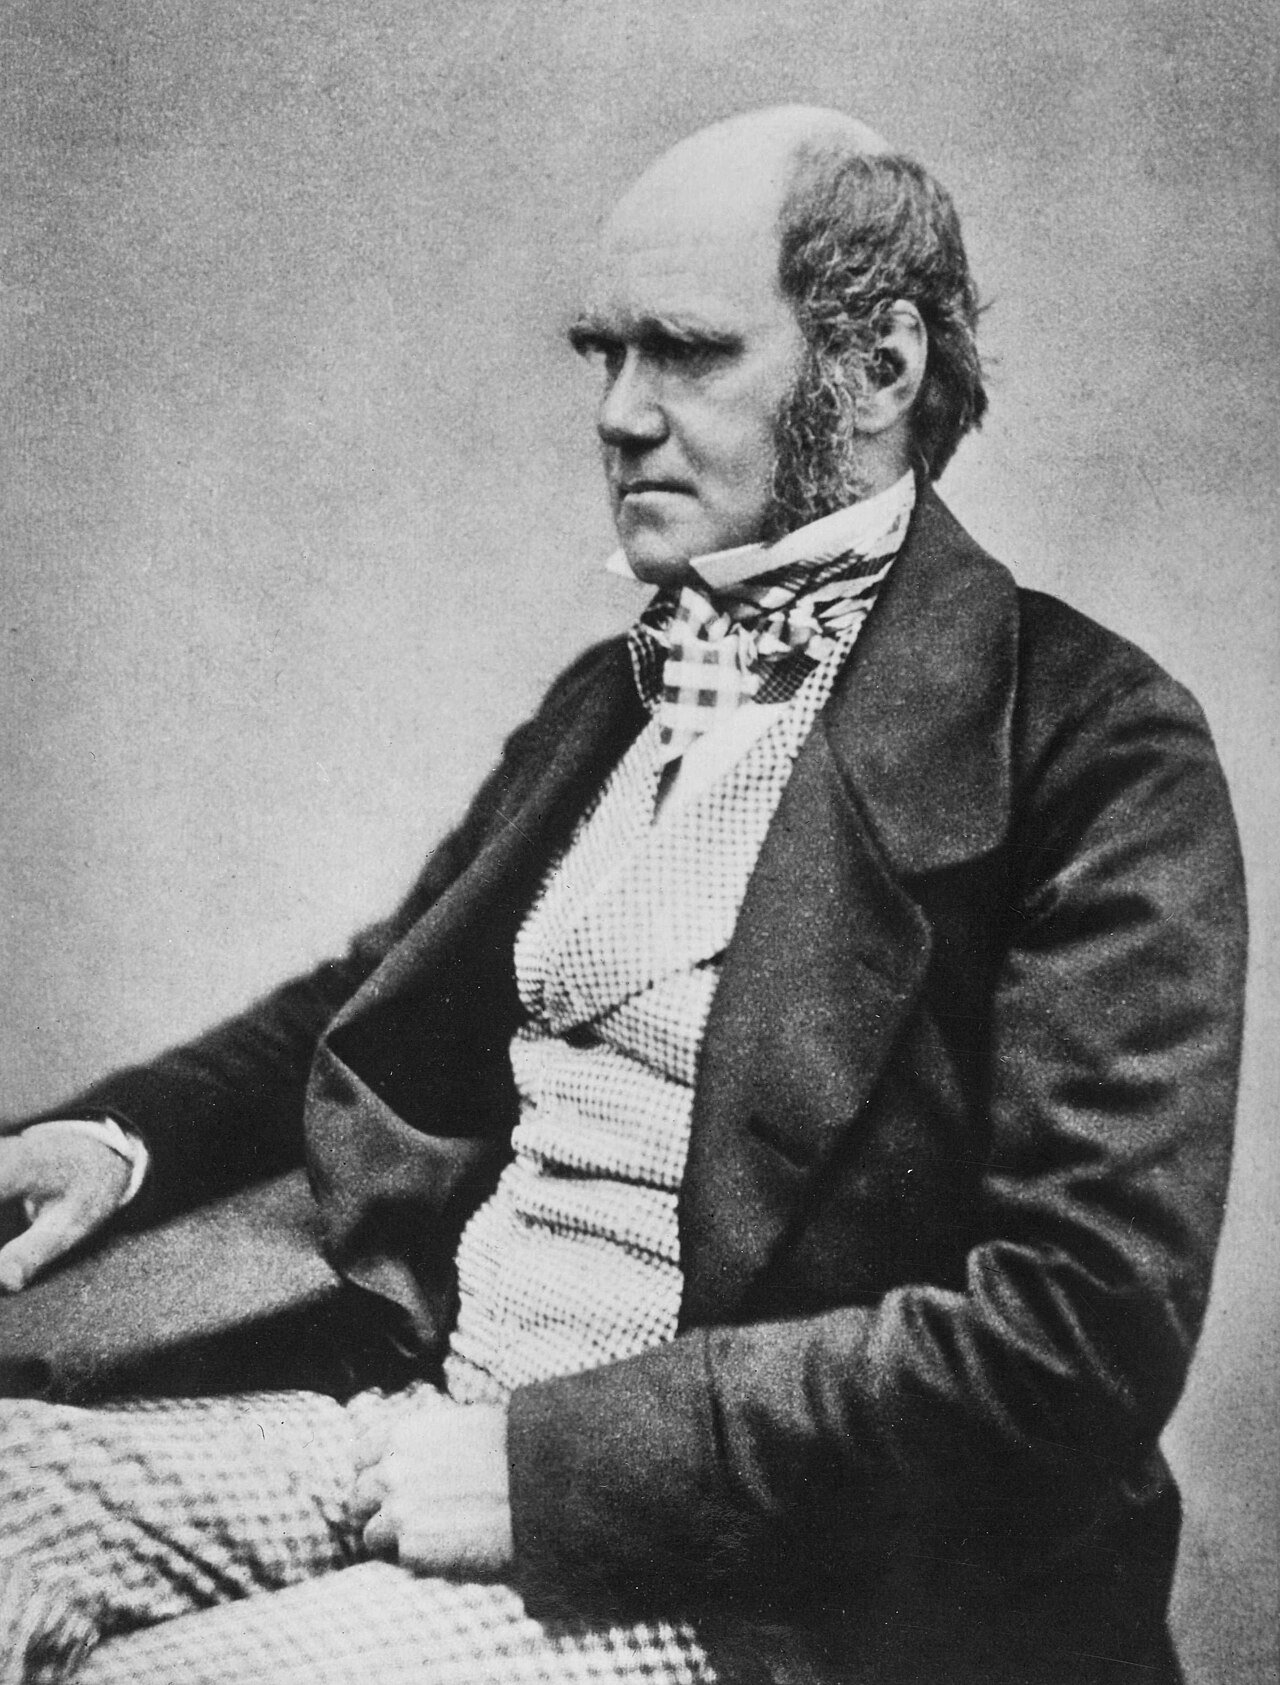
\includegraphics[width=0.36\linewidth]{images/book1/darwin.jpg}

{\small चार्ल्स डार्विन, जिन्होंने \omterm{def:g10:biodiversity-scales:species}{जातियों} की नातेदारी सबसे पहले किसी वृक्ष
की तरह खींची और वह क्रियाविधि प्रस्तावित की, यानी \omterm{def:g12:selection-drift-speciation:selection}{प्राकृतिक वरण}, जो उसे
उगाती है। फ़ोटो हेनरी मॉल और जॉन फ़ॉक्स, लगभग 1854, सार्वजनिक डोमेन।}
\end{omfigure}

\begin{remark}[वृक्ष क्या नहीं है]\label{rem:g12:phylogenetic-trees:not}
कोई वृक्ष इतिहास के बारे में एक परिकल्पना है, जो मौजूदा \omterm{def:g10:biodiversity-scales:species}{जातियों} से बनी है
और हर नए लक्षण तथा हर नए अनुक्रम से जाँची जाती है; वे असहमत हों तो वह
दोबारा खींचा जाता है, और वही दोबारा खींचना इस क्षेत्र का काम है। उसका कोई
ऊपरी सिरा नहीं है और प्रगति की कोई दिशा नहीं: मनुष्य लाखों में से एक सिरे
पर बैठे हैं, किसी और सिरे पर बैठी लैम्प्रे से न ऊँचे न अधिक पूरे। और उसके
किसी भी सिरे पर कोई पूर्वज नहीं है: पूर्वज वे गाँठें हैं, यानी बीत चुकी
\omterm{def:g12:selection-drift-speciation:population}{आबादियाँ}, जिनका होना वह वृक्ष अनुमानित करता है और जिनके जीवाश्म, जब मिलते
हैं, शाखाओं पर नहीं बल्कि उनके बग़ल में बैठते हैं।
\end{remark}

\section{अभ्यास}

\begin{exercise}[$\star$]\label{exo:g12:phylogenetic-trees:1}
किसी \omterm{def:g12:phylogenetic-trees:tree}{जातिवृत्तीय वृक्ष} के सिरे, उसकी गाँठें और उसका मूल क्या दर्शाते हैं?
\end{exercise}

\begin{exercise}[$\star$]\label{exo:g12:phylogenetic-trees:2}
पहले चित्र के वृक्ष A में छिपकली की सबसे क़रीबी नातेदार कौन-सी \omterm{def:g10:biodiversity-scales:species}{जाति} है?
मेंढक की?
\end{exercise}

\begin{exercise}[$\star$]\label{exo:g12:phylogenetic-trees:3}
किसी साझा व्युत्पन्न अवस्था की परिभाषा दीजिए और समझाइए कि कोई साझा पूर्वजी
अवस्था नातेदारी क्यों नहीं बताती।
\end{exercise}

\begin{exercise}[$\star$]\label{exo:g12:phylogenetic-trees:4}
\omterm{prop:g12:phylogenetic-trees:rules}{क्लेड} क्या है? क्या ``पक्षी'' एक \omterm{prop:g12:phylogenetic-trees:rules}{क्लेड} है? और ``सरीसृप'' (रोज़मर्रा के
अर्थ में)?
\end{exercise}

\begin{exercise}[$\star$]\label{exo:g12:phylogenetic-trees:5}
नर-वानर वाले वृक्ष से बताइए कि मनुष्य की सबसे क़रीबी नातेदार कौन-सी है, और
कौन-सी गाँठ सबसे पुरानी है।
\end{exercise}

\begin{exercise}[$\star\star$]\label{exo:g12:phylogenetic-trees:6}
पहले चित्र के वृक्ष A को ऊपर मनुष्य और नीचे मेंढक के साथ दोबारा खींचिए, और
जाँचिए कि हर नातेदारी अनबदली है।
\end{exercise}

\begin{exercise}[$\star\star$]\label{exo:g12:phylogenetic-trees:7}
दूसरे चित्र के आव्यूह में कबूतर (जबड़े 1, पाद 1, उल्ब 1, बाल 0, परों वाले
पंख 1) जोड़िए और उसे वृक्ष पर रखिए। ``परों वाले पंख'' लक्षण क्या जोड़ता है?
\end{exercise}

\begin{exercise}[$\star\star$]\label{exo:g12:phylogenetic-trees:8}
किसी डॉल्फ़िन के पास किसी शार्क जैसी धारारेखित देह तथा मीनपक्ष हैं, और बाल,
दूध तथा एक स्तनधारी जबड़ा भी। कौन-सा वृक्ष सबसे मितव्ययी है, और वे मीनपक्ष
क्या हैं?
\end{exercise}

\begin{exercise}[$\star\star$]\label{exo:g12:phylogenetic-trees:9}
घड़ी वाले चित्र की मदद से उन दो \omterm{def:g10:biodiversity-scales:species}{जातियों} के साझा पूर्वज को तिथि दीजिए जिनका
\omterm{def:g10:universal-dna:information}{DNA} 2.2\% में अलग है।
\end{exercise}

\begin{exercise}[$\star\star$]\label{exo:g12:phylogenetic-trees:10}
समझाइए कि ``चिंपैंज़ी हमारा पूर्वज है'' यह वाक्य उस वृक्ष को ग़लत क्यों
पढ़ता है, और सही वाक्य लिखिए।
\end{exercise}

\begin{exercise}[$\star\star$]\label{exo:g12:phylogenetic-trees:11}
दूसरे चित्र में लैम्प्रे को बाह्यसमूह की तरह क्यों इस्तेमाल किया गया है, और
उसकी जगह चूहा लिया जाए तो क्या बिगड़ जाएगा?
\end{exercise}

\begin{exercise}[$\star\star\star$]\label{exo:g12:phylogenetic-trees:12}
दो \omterm{def:g10:universal-dna:gene}{जीन} ऐसी तीन क़रीबी संबंधित \omterm{def:g10:biodiversity-scales:species}{जातियों} के लिए अलग-अलग वृक्ष देते हैं जो
एक-दूसरे से एक मिलियन साल के भीतर अलग हुईं। समझाइए कि यह किसी वृक्ष के
``ग़लत'' हुए बिना कैसे हो सकता है, और उसके लिए पूर्वज \omterm{def:g12:selection-drift-speciation:population}{आबादी} में
\omterm{def:g10:universal-dna:gene}{युग्मविकल्पियों} की फेंटाई इस्तेमाल कीजिए।
\end{exercise}

\begin{exercise}[$\star\star\star$]\label{exo:g12:phylogenetic-trees:13}
तेज़ी से विकसित होते किसी विषाणु की आणविक घड़ी 1\% प्रति साल चलती है; और
किसी स्तनधारी \omterm{def:g10:universal-dna:gene}{जीन} की 0.3\% प्रति मिलियन साल। समझाइए कि पहली किसी महामारी का
पीछा करने में और दूसरी स्तनधारियों के उद्गम को तिथि देने में क्यों
इस्तेमाल होती है, और कोई भी दूसरी का काम क्यों नहीं कर सकती।
\end{exercise}

\begin{exercise}[$\star\star\star$]\label{exo:g12:phylogenetic-trees:14}
दाँतों और लंबी हड्डीली पूँछ वाला किसी पक्षी का एक जीवाश्म 150 मिलियन साल
पुरानी चट्टानों में मिलता है। समझाइए कि वह वृक्ष की किसी शाखा के बग़ल में
क्यों रखा जाता है, किसी गाँठ पर क्यों नहीं, और वह उस गाँठ के बारे में क्या
बताता है।
\end{exercise}

\begin{exercise}[$\star\star\star$]\label{exo:g12:phylogenetic-trees:15}
``जीवन के वृक्ष के ऊपरी सिरे पर मनुष्य हैं।'' पढ़ने के नियमों, सिरों की
बराबर उम्र और सिरों की संख्या की मदद से एक अनुच्छेद में विवेचना कीजिए।
\end{exercise}

\section{समस्या: छह जातियाँ और एक घड़ी}

\begin{problem}[{सप्ताहांत समस्या --- एक वृक्ष दो बार बनाया गया, एक
लक्षण-तालिका से और DNA दूरियों से, दोनों की तुलना हुई, और गाँठों को तिथि
दी गई}]
\label{pb:g12:phylogenetic-trees:1}
छह \omterm{def:g10:biodiversity-scales:species}{जातियाँ}: शार्क, सामन, सैलामैंडर, मगरमच्छ, कबूतर, बिल्ली। बाह्यसमूह
लैम्प्रे है। लक्षण तालिका (1 = व्युत्पन्न):

\begin{center}
\small
\begin{tabular}{lcccccc}
 & हड्डीला कंकाल & चार पाद & उल्बी अंडा & परों वाले पंख & बाल & खोपड़ी का छिद्र \\ \hline
शार्क & 0 & 0 & 0 & 0 & 0 & 0 \\
सामन & 1 & 0 & 0 & 0 & 0 & 0 \\
सैलामैंडर & 1 & 1 & 0 & 0 & 0 & 0 \\
मगरमच्छ & 1 & 1 & 1 & 0 & 0 & 0 \\
कबूतर & 1 & 1 & 1 & 1 & 0 & 0 \\
बिल्ली & 1 & 1 & 1 & 0 & 1 & 1 \\
\end{tabular}
\end{center}

किसी एक \omterm{def:g10:universal-dna:gene}{जीन} के लिए \omterm{def:g10:universal-dna:information}{DNA} अंतर (\%):

\begin{center}
\begin{tabular}{lccccc}
 & सामन & सैलामैंडर & मगरमच्छ & कबूतर & बिल्ली \\ \hline
शार्क & 30 & 31 & 30 & 31 & 30 \\
सामन & & 24 & 25 & 25 & 24 \\
सैलामैंडर & & & 19 & 20 & 19 \\
मगरमच्छ & & & & 8 & 15 \\
कबूतर & & & & & 15 \\
\end{tabular}
\end{center}

\medskip
\noindent\textbf{भाग I --- लक्षणों से।}
\begin{enumerate}
  \item कौन-सी व्युत्पन्न अवस्था सबसे अधिक \omterm{def:g10:biodiversity-scales:species}{जातियाँ} साझा करती हैं? वह जो
        \omterm{prop:g12:phylogenetic-trees:rules}{क्लेड} तय करती है उसका और बाहर छूटी \omterm{def:g10:biodiversity-scales:species}{जातियों} का नाम लीजिए। (आख़िरी
        लक्षण खोपड़ी के बग़ल में वह इकलौता छिद्र है जो स्तनधारियों के पास
        होता है।)
  \item अगली सबसे व्यापक साझा अवस्थाओं के साथ आगे बढ़िए और एक-दूसरे में
        बैठे \omterm{prop:g12:phylogenetic-trees:rules}{क्लेड} सूचीबद्ध कीजिए।
  \item परों वाले पंख, बाल और खोपड़ी का छिद्र, हर एक किसी एक ही \omterm{def:g10:biodiversity-scales:species}{जाति} में
        मिलता है। क्या वे यह वृक्ष बनाने में मदद करते हैं? उन्हें
        उपयोगी क्या बनाता?
  \item वह वृक्ष खींचिए, और हर लक्षण उस शाखा पर लिखिए जहाँ वह प्रकट हुआ।
  \item इस तालिका के मुताबिक़ मगरमच्छ की सबसे क़रीबी नातेदार कौन-सी \omterm{def:g10:biodiversity-scales:species}{जाति}
        है? कौन-सी जोड़ी अकेली तालिका से नहीं सुलझाई जा सकती?
\end{enumerate}

\medskip
\noindent\textbf{भाग II --- \omterm{def:g10:universal-dna:information}{DNA} से।}
\begin{enumerate}[resume]
  \item \omterm{def:g10:biodiversity-scales:species}{जातियों} की किस जोड़ी की दूरी सबसे छोटी है? उन्हें पहले जोड़िए।
  \item उस जोड़ी से अगली कौन-सी \omterm{def:g10:biodiversity-scales:species}{जाति} जुड़ती है? वृक्ष पूरा होने तक आगे
        बढ़िए।
  \item \omterm{def:g10:universal-dna:information}{DNA} वाले वृक्ष की लक्षण वाले वृक्ष से तुलना कीजिए: वे कहाँ सहमत
        हैं, और \omterm{def:g10:universal-dna:information}{DNA} वह क्या तय कर देता है जो लक्षण नहीं कर सके?
  \item शार्क की बाक़ी सबसे दूरियाँ लगभग बराबर हैं। वृक्ष के आकार से
        समझाइए कि क्यों।
  \item मगरमच्छ--कबूतर दूरी (8) मगरमच्छ--बिल्ली दूरी (15) से छोटी है। यह
        रोज़मर्रा के समूह ``सरीसृप'' के बारे में क्या कहता है?
\end{enumerate}

\medskip
\noindent\textbf{भाग III --- वह घड़ी।}
जीवाश्म सैलामैंडर वंशरेखा के उल्बधारियों से अलग होने की तिथि 340 मिलियन साल
बताते हैं।
\begin{enumerate}[resume]
  \item सैलामैंडर--उल्बधारी दूरियों (लगभग 19\%) की मदद से उस घड़ी की दर
        प्रतिशत प्रति मिलियन साल में निकालिए। (दोनों वंशरेखाएँ बदलती रही हैं:
        वह दूरी दोनों शाखाओं के बदलाव गिनती है।)
  \item मगरमच्छ--कबूतर गाँठ को और उल्बधारी गाँठ को (मगरमच्छ/कबूतर बनाम
        बिल्ली) तिथि दीजिए।
  \item सामन गाँठ को और शार्क गाँठ को तिथि दीजिए।
  \item जीवाश्म मगरमच्छ--पक्षी बँटवारे के लिए लगभग 250 मिलियन साल और
        उल्बधारी बँटवारे के लिए 310 देते हैं। अपनी तिथियों से तुलना कीजिए
        और किसी \omterm{def:g10:universal-dna:gene}{एक-जीन} घड़ी की सटीकता पर टिप्पणी कीजिए।
  \item शार्क दूरियाँ (30--31\%) सामन वाली दूरियों (24--25\%) से मुश्किल
        से ही आगे जाती हैं, हालाँकि शार्क गाँठ कहीं पुरानी है। कोई
        व्याख्या प्रस्तावित कीजिए, और बताइए कि इस \omterm{def:g10:universal-dna:gene}{जीन} से बहुत पुरानी
        गाँठों को तिथि देने के लिए इससे क्या निकलता है।
\end{enumerate}

\medskip
\noindent\textbf{भाग IV --- पढ़ना और नाम देना।}
\begin{enumerate}[resume]
  \item अपने वृक्ष के वे \omterm{prop:g12:phylogenetic-trees:rules}{क्लेड} सूचीबद्ध कीजिए जिनमें बिल्ली है, सबसे छोटे
        से सबसे बड़े तक।
  \item क्या ``मछलियाँ'' (शार्क और सामन) एक \omterm{prop:g12:phylogenetic-trees:rules}{क्लेड} हैं? और ``उल्बधारी''?
        उचित ठहराइए।
  \item कोई विद्यार्थी कहता है कि सैलामैंडर ``मछलियों और सरीसृपों के बीच
        की कोई मध्यवर्ती चीज़'' है। उस कथन को वृक्ष की भाषा में ठीक कीजिए।
  \item हड्डीले कंकाल, चार पादों और बिना किसी उल्बी अंडे वाला एक जीवाश्म
        मिलता है, जिसकी तिथि 360 मिलियन साल है। वह वृक्ष के मुक़ाबले कहाँ
        बैठता है, और उसकी तिथि किस बात की पुष्टि करती है?
  \item परिणाम लिखिए: छहों \omterm{def:g10:biodiversity-scales:species}{जातियों} का वृक्ष (एक-दूसरे में बैठे कोष्ठकों के
        रूप में), वह एक नातेदारी जो \omterm{def:g10:universal-dna:information}{DNA} ने तय की, और मगरमच्छ--कबूतर
        बँटवारे की आकलित तिथि।
\end{enumerate}
\end{problem}
